\section{Algorithm}
As we all know, one word may have multiple translations in another language, and our extension is expected to select the most appropriate one based on the context.We call such translation selection as cross-lingual word sense disambiguation (WSD).
\\
WSD is an open problem in natural language processing and ontology, aiming at identifying the proper sense of a word (i.e. meaning) in a context, when the word has multiple meanings. However, the system that I have implemented is  different from the traditional WSD. Normally, WSD is to identify its sense in its original language, but my system is to identify its sense in another language.
\\
It has been proved by a lot of studies that context is the key to learning a new language. This further suggests that a good word sense disambiguation system is necessary for our Chrome Extension. It can help user remember vocabulary efficiently and is a key feature that differentiate our software from other language learning tools.
\\
In this following, I describe four approaches that I have tried to accomplish WSD system, which is also my main progress in the second semester. The four approaches are: 
% Tao: Please give a short definition for other three methods.
\begin{itemize}
\item Frequency based: always selecting the most frequent translation (the baseline),
\item Part-of-Speech Tag based: selecting the translation based on the Part-of-Speech Tag of the English word
\item Translation based: Selecting the translation based on the result from existing Machine Translation systems
\item Category based: Selecting the translation based on the category of the news article
\end{itemize}

\subsection{Baseline}
The simplest way to select a translation from the candidates is by random. However, the correctness of this method is very low, probably less than 20\%, and is not a good baseline for other methods to compete with. Another simple idea is to always select the most commonly used translation. Luckily, when I crawled the dictionary, Google Translate does provide usage frequency of each Chinese Translation.  This turns out to be a much better result, and thus serves as a fair baseline method.
\\
\subsection{Part-of-Speech Tagger}
As we all know, many English words have more than one Part-of-Speech (POS) tags and their Chinese translations in different POS may differ a lot. For example, the word ``book" has two POS tags, noun and verb. If it is used as a noun, mostly it means a handwritten or printed work of fiction or nonfiction, which should be translated as ``书", and mostly means to reserve if used as a verb, which should be translated as ``预定". Therefore, if I can get the POS tag of the English word, it might help me identify its sense or the Chinese translation.

\begin{table}[ht]
    \caption{Sample input/output of POSTagger}
    \label{table:part_of_speech}
    \begin{center}
    \begin{tabular}{| p{1.5cm} | p{2.5cm} | p{2.2cm} |}
        \hline
        Input & Output & Tag Description \\
        \hline
        They are treating me like family now & They|PRP are|VBP treating|VBG me|PRP like|IN family|NN now|RB & IN | preposition or conjunction\\
        \hline
    \end{tabular}
    \end{center}
\end{table}

Among all possible on-line sources, Stanford Log-linear Part-of-Speech Tagger~\cite{Toutanova2003} is the most stable and well performed Part-of-Speech Tagger, which is developed by The Stanford Natural Language Processing Group. Column one and column two of Table~\ref{table:part_of_speech} is one sample input and output. However, the tag from Part-of-Speech Tagger is not the one we normally used. I need one more step to match the tag to its Part-of-Speech. Therefore, I followed the Part-of-Speech guidelines from the University of Pennsylvania (Penn) Treebank Tag-set. The last column of Table \ref{table:part_of_speech} is one example of the matching.

\begin{algorithm}[ht]
\caption{Part-of-Speech Tagger}
\label{algorithm:wsd_1}
\begin{algorithmic}
\REQUIRE POS Tagger, Dictionary \textless English, Chinese, POS \textgreater, Input English

\STATE{$Pairs<word,POS> \leftarrow POSTagger \leftarrow English$}

\IF{$EnglishWord \subset Dictionary.English$}
    \STATE{$TranslationList \leftarrow Dictionary.Chinese+Dictionary.POS$}
    \FOR{$word \subset Pairs.word$}
        \IF{$word = EnglishWord$}
            \STATE{$POSResult \leftarrow Pairs.POS$}
            \STATE{$Break$}
        \ENDIF
    \ENDFOR
    \FOR{$POS \subset TranslationList.POS$}
        \IF{$POS = POSResult$}
            \STATE{$FinalResult \leftarrow TranslationList.Chinese$}
            \STATE{$Break$}
        \ENDIF
    \ENDFOR
\ENDIF
\RETURN FinalResult
\end{algorithmic}
\end{algorithm}
\\
\begin{table}[ht]
    \caption{Example input/output of POSTagger}
    \label{table:part_of_speech_example}
    \begin{center}
    \begin{tabular}{| p{2.5cm} | p{4cm} |}
        \hline
        Input English & they are treating me like family now\\
        \hline
        English Word & like \\
        \hline
        Translation List & \parbox[t]{4cm}{verb : 喜欢, 爱, 爱好, 待见, 好, 看上, 喜, 喜爱, 喜好\\ adjective : 一样, 似, 同, 相似\\ conjunction : 如同\\noun : 类\\preposition : 好像, 好比, 好以\\adverb : 不啻, 若}\\
        \hline
        Pairs \textless word,POS\textgreater & they|PRP are|VBP treating|VBG me|PRP like|IN family|NN now|RB\\
        \hline
        Final Result & 好像\\
        \hline
    \end{tabular}
    \end{center}
\end{table}

Algorithm \ref{algorithm:wsd_1} is the approach of using POSTagger. From Algorithm  \ref{algorithm:wsd_1}, firstly, if the word "like" need to be translated, the algorithm will fetch all the Chinese translations as well as their Part-of-Speech tag from our dictionary. Secondly, the algorithm will send the original English sentence to Part-of-Speech Tagger, which is a Java package and has been wrapped into a server. After the client has got the output from the server, it will fetch the corresponding tag and match it to Part-of-Speech tag based on the guidelines mentioned above. Lastly, it will select the translations based on the POS.
\\
In most cases, this algorithm is only a filter. There might be a few Part-of-Speech tags matched from the output and one POS tag might have a few corresponding Chinese translations. In this case, I will choose the translation with the highest frequency of use, which is actually a combination of POSTagger and baseline, so that this system is testable independently.



\subsection{Machine Translation}
Since our target is to select the most appropriate translation based on the context, using existing Machine Translation (MT) systems is also a good approach, as all of them will certainly translate words based on the context.
\\
There are mainly two kinds of MT systems. One is off-line Machine Translation systems, which are mostly not available as mostly they are build for internal usage. Luckily, NUS NLP group built one MT system before, and it has been wrapped into a server, so that I can use it as an on-line service. The other one is on-line MT system, which are wrapped as a server and open to public, such as Bing Translator or Google Translate. As only Bing Translator is free, I decide to try Bing Translator as well.
\\
The first priority of choosing a MT system is its translation quality, if it can give me a result that nearly as good as a result from human translation, then the Chinese word that I generated from the MT system will have a high chance to be correct as well. However, after I tried both MT systems, the performance of the one from NLP group is worse than Bing Translator and the server is very unstable, I decide to use Bing Translator as my Machine Translation system.
\\

\subsubsection{Bing}
\begin{table}[ht]
    \caption{Example input/output of Bing Translator}
    \label{table:bing_translator}
    \begin{tabular}{| p{4cm} | p{2.8cm} |}
        \hline
        Input & Output \\
        \hline
        including a 45-caliber pistol a pump shotgun and an ar-15 rifle & 包括 45 口径手枪唧筒式猎枪和 ar-15 步枪\\
        \hline
        they are asking for privacy at this time & 在这个时候他们正在寻求隐私\\
        \hline
        possessing cartridges used exclusively by the military and carrying a firearm without a license & 拥有只供军方使用的墨盒和携带火器的许可证\\
        \hline
    \end{tabular}
\end{table}
Bing Translator, also called Microsoft Translator, is a on-line Machine Translation system that developed by Microsoft team with a cloud-based API that is conveniently integrated into multiple products, tools, and solutions. Table \ref{table:bing_translator} is the sample input and output of Bing Translator.
\\
\begin{algorithm}[ht]
\caption{Bing Translator}
\label{algorithm:wsd_3}
\begin{algorithmic}
\REQUIRE Bing Translator, Dictionary \textless English, Chinese\textgreater, Input English
\STATE{$ChineseTranslation \leftarrow Bing Translator \leftarrow English$}
\IF{$EnglishWord \subset Dictionary.English$}
    \STATE{$TranslationList \leftarrow Dictionary.Chinese$}
    \STATE{$MaxLength = 0$}
    \FOR{$ChineseWord \subset TranslationList.Chinese$}
        \IF{$(ChineseWord \subset ChineseTranslation) \cap (MaxLength < ChineseWord.Length)$}
            \STATE{$FinalResult \leftarrow ChineseWord$}
        \ENDIF
    \ENDFOR
\ENDIF
\RETURN FinalResult
\end{algorithmic}
\end{algorithm}
\begin{table}[ht]
    \caption{Example input/output of Bing Translator}
    \begin{center}
    \begin{tabular}{| p{2.5cm} | p{4cm} |}
        \hline
        Input English & including a 45-caliber pistol a pump shotgun and an ar-15 rifle\\
        \hline
        English Word & pump \\
        \hline
        Translation List & \parbox[t]{4cm}{verb:抽, 抽水, 打气, 唧, 唧筒, 套\\ noun:抽水机, 唧筒}\\
        \hline
        Chinese Translation & 包括 45 口径手枪唧筒式猎枪和 ar-15 步枪\\
        \hline
        Final Result & 唧筒\\
        \hline
    \end{tabular}
    \end{center}
\end{table}
%\begin{figure}[ht]
%   \centering
%   \includegraphics[width=0.9\textwidth]{wsd_5.jpg}
%   \caption{Steps of using Bing Translator}
%   \label{fig:wsd_5}
%\end{figure}

Algorithm \ref{algorithm:wsd_3} is the steps of using Bing Translator. The original English sentence is ``including a 45-caliber pistol a pump shotgun and an ar-15 rifle" and ``pump" is the word that we want to translate. Firstly, this algorithm will fetch all the Chinese translations from the database. Next, it will send the original English sentence to Bing Translator using the API provided by Microsoft and get the result that returned from Bing Translator. After that, for each Chinese translation, I will check whether this translation is a substring of the Bing Translator result. If there are a few translations that can match with the Bing Translator result, I will select the longest translation. If there are a few translations with the same length and all of them can match with the Bing Translator result, I will select the translation with the highest frequency of use. In this example, both ``唧" and ``唧筒" are the substrings of Bing Translator result. As ``唧筒" have two characters and ``唧" only have one character, this algorithm will take ``唧筒" as the final result.


\subsubsection{Bing+}
\begin{table}[ht]
    \caption{Another example of Bing Translator}
    \label{table:bing_plus_1}
    \begin{center}
    \begin{tabular}{| p{2.5cm} | p{4cm} |}
        \hline
        Input English & as a result of the latest premier league broadcast rights deal all of its teams have made it into the worlds top 40 clubs\\
        \hline
        English Word & top \\
        \hline
        Translation List & \parbox[t]{4cm}{顶部, 顶端, 顶, 颠, 盖, 极, 尖, 尖峰, 面, 上身, 头, 上面的, 最大的, 最高的, 盖}\\
        \hline
        Chinese Translation & 由于最新英超联赛转播的权交易所有其团队已经进入世界顶级40名俱乐部\\
        \hline
        Final Result & 顶\\
        \hline
    \end{tabular}
    \end{center}
\end{table}
Table \ref{table:bing_plus_1} is another example of Bing Translator. In this example, ``top" is the word that need to be translated. If we manually translated the word ``top" based on the Bing Translator, I would say the correct translation should be ``顶级". However, the word ``顶级" is not covered by our dictionary, so the final result generated by Bing algorithm is ``顶" as this is the only word that matches Bing Translator. Although the meaning of the word ``顶" is almost the same as that of the word ``顶级" and I, personally, would prefer to make ``顶" as one of the correct result when I tried to evaluate this example, the word ``顶级" is more accurate in this context. Therefore, is there any way to solve this problem and make the result more accurate? Yes, solving this problem requires our system to generate Chinese words that are not covered by our dictionary and the only way is to use Word Segmenter.
\\
\begin{table}[ht]
    \caption{Example of Stanford Word Segmenter}
    \label{table:bing_plus_2}
    \begin{tabular}{| p{3.5cm} | p{3.5cm} |}
        \hline
        Input & Output\\
        \hline
        问题是你将要运行直赫顿到他说的第一修正案 & 问题, 是, 你, 将要, 运行, 直赫顿, 到, 他, 说的, 第一, 修正案\\
        \hline
        博士苏斯博士知道这将是他出版的最后一本书 & 博士, 苏, 斯, 博士, 知道, 这, 将, 是, 他, 出版, 的, 最后, 一, 本, 书\\
        \hline
        进入世界顶级40名俱乐部 & 进入, 世界, 顶级, 40, 名, 俱乐部\\
        \hline
    \end{tabular}
\end{table}
\\
Text segmentation is the process of dividing written text into meaningful units, such as words, sentences, or topics. The term applies both to mental processes used by humans when reading text, and to artificial processes implemented in computers, which are the subject of natural language processing. I use Stanford Word Segmenter to do Chinese text segmentation. Stanford Word Segmenter is a open source Java package that developed by The Stanford Natural Language Processing Group. I wrapped it into a local server and Table \ref{table:bing_plus_2} contains some example of the input and output of Stanford Word Segmenter.
\\
\begin{algorithm}[ht]
\caption{Bing+}
\label{algorithm:wsd_4}
\begin{algorithmic}
\REQUIRE Bing Translator, Word Segmenter, Dictionary \textless English, Chinese\textgreater, Input English
\STATE{$ChineseTranslation \leftarrow Bing Translator \leftarrow English$}
\STATE{$SegmentedChineseTranslation \leftarrow Word Segmenter \leftarrow ChineseTranslation$}
\IF{$EnglishWord \subset Dictionary.English$}
    \STATE{$TranslationList \leftarrow Dictionary.Chinese$}
    \STATE{$MaxLength = 0$}
    \FOR{$ChineseWord \subset TranslationList.Chinese$}
        \IF{$(ChineseWord \subset ChineseTranslation) \cap (MaxLength < ChineseWord.Length)$}
            \STATE{$FinalResult \leftarrow ChineseWord$}
        \ENDIF
    \ENDFOR
    \FOR{$SegmentedWord \subset SegmentedChineseTranslation$}
        \IF{$FinalResult \subset SegmentedWord$}
            \STATE{$FinalResult \leftarrow SegmentedWord$}
        \ENDIF
    \ENDFOR
\ENDIF
\RETURN FinalResult
\end{algorithmic}
\end{algorithm}
\\
\begin{table}[ht]
    \caption{Example input/output of Bing+}
    \begin{center}
    \begin{tabular}{| p{2.5cm} | p{4cm} |}
        \hline
        Input English & as a result of the latest premier league ... have made it into the worlds top 40 clubs\\
        \hline
        English Word & top \\
        \hline
        Translation List & \parbox[t]{4cm}{顶部, 顶端, 顶, 颠, 盖, 极, 尖, 尖峰, 面, 上身, 头, 上面的, 最大的, 最高的, 盖}\\
        \hline
        Chinese Translation & 由于, 最新, 英, 超联赛, 转播, 的, 权 ... 进入, 世界, 顶级, 40, 名, 俱乐部\\
        \hline
        Final Result & 顶级\\
        \hline
    \end{tabular}
    \end{center}
\end{table}

\\
Algorithm \ref{algorithm:wsd_4} is the approach of using Bing Translator together with Stanford Word Segmenter, and I would like to use Bing+ to represent this algorithm. Step one, two and three has been described in the previous section as it is exactly the same as Bing approach. From Bing approach, this algorithm will generate ``顶" as the result. After that, Bing+ approach will send the Chinese sentence returned from Bing Translator to Stanford Word Segmenter. Then, this algorithm will use the segmented word that contains the Bing result as a substring or equals to the Bing result as the final result. In this example, the final result of Bing+ is ``顶级" which is the best result that can be generated from the result of Bing Translator and also a result that does not covered by our dictionary.
\\
\subsubsection{Bing++}
\begin{table}[ht]
    \caption{Another example of Bing+ Translator}
    \label{table:bing_plus_plus_1}
    \begin{center}
    \begin{tabular}{| p{2.5cm} | p{4cm} |}
        \hline
        Input English & but the world no 46 played one of his best matches crucially not crumbling when the finish line was in sight\\
        \hline
        English Word & line \\
        \hline
        Translation List & \parbox[t]{4cm}{线, 线路, 路线, 系, 行列, 划线于, 衲, 排, 诗句, 纹, 线条, 衬, 衲}\\
        \hline
        Chinese Translation & 但, 世界, 没有, 46, 起, 最, 重要, 的, 是, 不, 崩溃, 在, 终点, 线上, 视线, 的, 时候, 他, 最, 好, 的, 比赛, 之一\\
        \hline
        Final Result & 线上 or 视线\\
        \hline
    \end{tabular}
    \end{center}
\end{table}
Table \ref{table:bing_plus_plus_1} is another example of Bing+ Translator. In this example, ``line" is the word that need to be translated and the correct translation based on Bing Translator should be ``线上". The Bing approach will get ``线" as the result. After the Bing approach got the result, the next step should be finding the segmented word that contains ``线" as a substring. However, both word ``线上" and word ``视线" contains word ``线" as a substring and, obviously, only the word ``线上" is the correct result and ``视线" is actually the translation for English word ``sight". As both results generated by Bing+ approach are not covered by our dictionary, the algorithm cannot get the frequency of use information. As a result, Bing+ approach will randomly choose one word, so there is only 50\% to get the correct result. Is there any way to solve this problem and always choose the correct result in this case? Yes, as long as the algorithm could get the word alignment information, it will know exactly how to match the Chinese words with those English words.
\\
\begin{table}[ht]
    \caption{Example input/output of Word Alignment}
    \label{table:bing_plus_plus_2}
    \begin{center}
    \begin{tabular}{| p{1.5cm} | p{5cm} |}
        \hline
        Input_1 & dr seuss knew it would be the last book he published\\
        \hline
        Output_1 & 博士苏斯博士知道这将是他出版的最后一本书\\
        \hline
        Output_1 & 0:1|0:1 3:7|2:5 9:12|6:7 14:15|8:8 17:21|9:9 23:24|10:10 26:28|14:14 30:33|15:17 35:38|18:19 40:41|11:11 43:51|12:13 \\
        \hline
        Input_2 & the problem is youre going to run straight headon into the first amendment he said \\
        \hline
        Output_2 & 问题是你将要运行直赫顿到他说的第一修正案\\
        \hline
        Output_2 & 4:10|0:1 12:13|2:2 15:19|3:3 21:28|4:5 30:32|6:7 34:41|8:8 43:48|9:10 50:53|11:11 59:63|15:16 65:73|17:19 75:76|12:12 78:81|13:13 \\
        \hline
        Input_3 & this is something preschoolers deal with all the time\\
        \hline
        Output_3 & 这是学龄前儿童处理所有的时间\\
        \hline
        Output_3 & 0:3|0:0 5:16|1:1 18:29|2:6 31:39|7:8 41:43|9:10 45:47|11:11 49:52|12:13\\
        \hline
    \end{tabular}
    \end{center}
\end{table}
\\
Bitext word alignment or simply word alignment is the natural language processing task of identifying translation relationships among the words (or more rarely multiword units) in a bitext, resulting in a bipartite graph between the two sides of the bitext, with an arc between two words if and only if they are translations of one another. I use Bing Word Alignment API\footnote{\url{https://msdn.microsoft.com/en-us/library/dn198370.aspx}} developed by Microsoft team to get the word alignment from English to Chinese Simplified. Luckily, although this API only support very few sets of language pairs, English to Chinese Simplified is one of the few supported sets. Table \ref{table:bing_plus_plus_2} has some examples of input and output from Bing Word Alignment. The left column is the original English sentence, the column in the middle is the translated Chinese sentence and the right column is the word alignment information. For word alignment information, the colon separates start and end index, the dash separates the languages, and space separates the words. For example, in the second column, ``0:1|0:1" means the word ``dr" should match with word ``博士" and ``9:12|6:7" means the word ``knew" should match with word ``知道".

\begin{algorithm}[ht]
\caption{Bing++}
\label{algorithm:wsd_5}
\begin{algorithmic}
\REQUIRE Bing Translator, Word Segmenter, Word Alignment, Dictionary \textless English, Chinese\textgreater, Input English
\STATE{$ChineseTranslation \leftarrow Bing Translator \leftarrow English$}
\STATE{$SegmentedChineseTranslation \leftarrow Word Segmenter \leftarrow ChineseTranslation$}
\STATE{$Pair<EnglishWord,ChineseWord> \leftarrow Word Alignment \leftarrow English$}
\IF{$EnglishWord \subset Dictionary.English$}
    \STATE{$TranslationList \leftarrow Dictionary.Chinese$}
    \STATE{$MaxLength = 0$}
    \FOR{$ChineseWord \subset TranslationList.Chinese$}
        \IF{$(ChineseWord \subset ChineseTranslation) \cap (MaxLength < ChineseWord.Length)$}
            \STATE{$FinalResult_1 \leftarrow ChineseWord$}
        \ENDIF
    \ENDFOR
    \FOR{$SegmentedWord \subset SegmentedChineseTranslation$}
        \IF{$FinalResult_1 \subset SegmentedWord$}
            \STATE{$FinalResult_1 \leftarrow SegmentedWord$}
        \ENDIF
    \ENDFOR
    \FOR{$Word \subset Pairs.EnglishWord$}
        \IF{$EnglishWord = Word$}
            \STATE{$FinalResult_2 \leftarrow Pairs.ChineseWord$}
        \ENDIF
    \ENDFOR
\ENDIF
\RETURN $FinalResult_1 \cup FinalResult_2$
\end{algorithmic}
\end{algorithm}

\begin{table}[ht]
    \caption{Example input/output of Bing++}
    \begin{tabular}{| p{4cm} | p{1.2cm} | p{2.3cm} | p{3.5cm} | p{1.5cm} | p{1.5cm} |}
        \hline
        Input English & English Word & Dictionary Chinese & Chinese Translation & Bing+ & Bing++ \\
        \hline
        state department spokeswoman jen psaki said that the allies had a long history of cooperation & top & ...陈, 陈说, 称, 称述, 发表, 发言... & 国家, 部门, 的, 女, 发言人, jenpsaki, 说, 盟国, 有, 很, 长, 的, 合作, 历史 & 发言人 & 国家 \\
        \hline
    \end{tabular}
\end{table}
%\begin{figure}[ht]
%   \centering
%   \includegraphics[width=0.9\textwidth]{wsd_7.jpg}
%   \caption{Steps of Bing++}
%   \label{fig:wsd_7}
%\end{figure}


Algorithm \ref{algorithm:wsd_5} is the approach of using Bing+ approach together with the Microsoft Bing Word Alignment. First few steps are exactly the same as Bing+ approach. In this example, ``state" is the word that need to be translated. The result from Bing+ approach is ``发言人", which is the translation of ``spokeswoman", because the Chinese translation ``发言" can be translated from both ``state" and ``spokeswoman". Then step five will send the original English sentence to Bing Word Alignment. Now, there will be two final results, one from Bing+ approach and the other one from Bing Word Alignment and the algorithm will choose the correct one from these two results. In this example, ``state" will match with ``国家" and the algorithm will choose ``国家" as the final result as well.


\begin{table}[ht]
    \caption{Some examples of Bing+ and Bing++}
    \label{table:bing_plus_plus_3}
    \begin{tabular}{| p{5cm} | p{5cm} | p{2cm} | p{2cm} |}      
        \hline
        English & Chinese & Bing+ & Bing++ \\
        \hline
        oh the places youll go! rose to the bestseller list shortly after it was released in 1990 and continues to pop up there most every spring as high school and college grads transition to a new phase of life & 哦你要去的地方!升至畅销书排行榜之后不久它于1990年被释放并继续弹出那里大多数每年春天为高中和大学毕业生过渡到人生的一个新阶段 & 春天 & 年春天\\
        \hline
        the darkness of the book is what makes the optimism credible nel said & 这本书的黑暗是什么使乐观可信nel说 & 书 & 本书\\
        \hline
        other seuss books have emerged since his death in 1991 but this was the last he had a hand in & 自从他死后在1991年出现了其他苏斯博士的书,但这是他一只手在最后一次 & 最后 & 最后一次\\
        \hline
    \end{tabular}
\end{table}

One general question about this approach is that, since I can get the official word alignment from Bing Word Alignment approach, is Bing+ approach still useful? Table \ref{table:bing_plus_plus_3} contains some examples of Bing+ approach and Bing++ approach. From left to right, the four columns are original English sentence, Chinese translation, result from Bing+ approach and result from Bing++ approach. It is very obvious that the result from Bing+ approach is the substring of the result from Bing++ approach, but which one is better? As the purpose of our Word Sense Disambiguation system is to select the most appropriate translation based on the context, but Bing Translator is a bit too smart comparing with our purpose. Bing Translator will generate some Chinese words that cannot be translated from any of the English word but can make this sentence clear and smooth. In this case, our system will choose the short answer instead of the long answer. That's why in the Bing++ approach, I will keep the result both from Bing+ approach and Bing Word Alignment and choose the better one.
\\

\subsection{News Category}
The word ``interest" have two very different translations when it is used as a noun. One translation is ``the feeling of a person whose attention, concern, or curiosity is particularly engaged by something", which should be translated as ``兴趣". The other translation is ``a share, right, or title in the ownership of property, in a commercial or financial undertaking, or the like", which should be translated as ``利益". It is quite obvious that the second sense is mostly used in financial related topics. Therefore, if we can analyze the category of the original article and 
select the translation with the same category label, it might help disambiguate the word meaning.
\\
Getting the category of the original news article is very simple. Most news websites have a manually assigned a category for each news article and in most cases, the category label is part of the URL.
\\
However, assigning a category for Chinese word is not simple. As we are dealing with news, it is good to obtain such information from Chinese news domain. I crawled 100 Chinese news articles in each category from  Baidu News\footnote{\url{http://news.baidu.com/}}, making around 1000 news articles in total. After I got all the news articles, I send all the news articles to the Stanford Chinese Word Segmenter, and further calculate word document frequency under each  category. For example, if word ``interest" is found five times in article A and three times in article B, both article A and B are under ``finance" category, then I will add two for category ``finance" of word ``interest" as it will be counted only once even it can be found multi times in one article. I will use ``weight" to represent this value and ``averageweight" is the average weight of all categories of one word. After that, I will normalize the weight and use Equation~\ref{equation:category_1} and Equation~\ref{equation:category_2} to assign categories for those Chinese words. Basically, the two equations means that, if this word can be found in at least ten different news articles and more than 80\% of the articles are under the same category, then I will use this category for this word.

\begin{equation}
averageweight > 1\\
\label{equation:category_1}
\end{equation}
\begin{equation}
threshold > 8 * averageweight\\
\label{equation:category_2}
\end{equation}

\begin{figure}[ht]
    \centering
    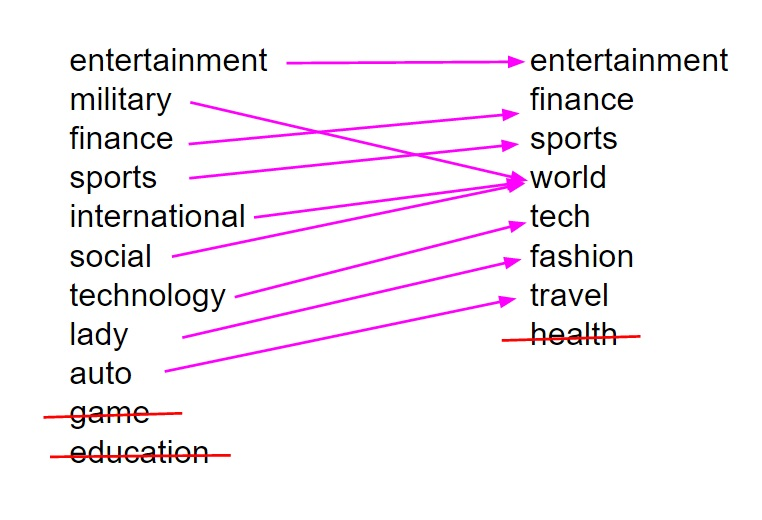
\includegraphics[width=0.9\textwidth]{wsd_4.jpg}
    \caption{Alignment between categories}
    \label{fig:wsd_4}
\end{figure}

However, the categories in Chinese and English news are not the same.
I manually aligned the categories and delete some categories when necessary.
As shown in Figure \ref{fig:wsd_4}, 
on the left side, the 11 categories are from Chinese news website and on the right side, the eight categories are from English news website. 
During the alignment, I not only take the name of category into account, but also consider the semantics of the category.
\\
\begin{algorithm}[ht]
\caption{News Category}
\label{algorithm:wsd_2}
\begin{algorithmic}
\REQUIRE Dictionary \textless English, Chinese, category\textgreater, Input English, News URL

\IF{$EnglishWord \subset Dictionary.English$}
    \STATE{$TranslationList \leftarrow Dictionary.Chinese+Dictionary.category$}
    \STATE{$EnglishCategory \leftarrow URL.category$}
    \FOR{$category \subset TranslationList.category$}
        \IF{$category = EnglishCategory$}
            \STATE{$FinalResult \leftarrow TranslationList.Chinese$}
            \STATE{$Break$}
        \ENDIF
    \ENDFOR
\ENDIF
\RETURN FinalResult

\end{algorithmic}
\end{algorithm}
\begin{table}[ht]
    \caption{Example input/output of News Cateogry}
    \begin{tabular}{| p{4cm} | p{1.5cm} | p{3cm} | p{3cm} | p{2cm} |}
        \hline
        Input English & English Word & Dictionary.Chinese & Category & FinalResult \\
        \hline
        duncan told cnns don lemon hes just painting a picture of urban street life with his lyrics & picture & ... 相, 影, 影片(entertainment), 帧, 想象, 画 ... & entertainment & 影片 \\
        \hline
    \end{tabular}
\end{table}
%\begin{figure}[ht]
%   \centering
%   \includegraphics[width=0.9\textwidth]{wsd_3.jpg}
%   \caption{Steps of using news category}
%   \label{fig:wsd_3}
%\end{figure}
\\
Algorithm \ref{algorithm:wsd_2} is the steps of using news category. The English sentence is the original sentence and ``picture" is the word that need to be translated. Firstly, the algorithm will fetch all the Chinese translations for word ``picture" and split them with comma. In this example, only the word ``影片" has a category ``entertainment". Next, the algorithm will fetch the category of the English news article from the URL, which is also ``entertainment".
In this case, the algorithm will use ``影片" as the translation for word ``picture". If a few words shares the same category, the algorithm will choose the translation with the highest frequency of use.